\documentclass[a4paper,14pt]{article}

\title{report}
\author{Зарубин Всеволод}
\date{today}
\usepackage[T2A]{fontenc}
\usepackage[utf8]{inputenc}
\usepackage[english,russian]{babel}
\usepackage{amsmath,amsfonts,amssymb,amsthm,mathtools,bpchem}
\usepackage{fancyhdr}
\usepackage{indentfirst}
\usepackage{float}
\usepackage{etaremune}

\usepackage[margin=1in]{geometry}

\pagestyle{fancy}
\fancyhf{}
\rhead{\thepage}
\renewcommand{\headrulewidth}{0pt}

\thispagestyle{empty}


\begin{document}
\begin{titlepage}
\begin{center} 
 
\large Московский физико-технический институт\\
Факультет молекулярной и химической физики\\
\vspace{6.5cm}
\Large Задание по курсу \\ Вычислительная математика\\
\textbf{\Large Гиперболические системы уравнений}\\
\end{center} 

\vspace{7cm}
{\par 
	\raggedleft \large 
	\emph{Выполнил}\\ 
	студент 3 курса\\ 
	643 группы ФМХФ\\ 
	Зарубин Всеволод 
\par}
\begin{center}
\vfill \today
\end{center}
\end{titlepage}
\newpage
\setcounter{page}{2}

\newpage
	\section{Постановка задачи}
    \Large Необходимо численно решить систему линейных \\гиперболических уравнений.\\
    \subsection{Параметры задачи}
    Используются разностные схемы:
    \begin{center}
    \begin{enumerate}
        \item Схема Куранта-Изаксона-Риса
        \item Гибридная схема Федоренко. \\
        Порядок схемы изменяется от второго в областях\\
        гладкости решения, до первого в областях больших градиентов.  
    \end{enumerate}
    \end{center}
    \vspace{0.5cm}
    Модельное уравнение:\\
    \begin{equation}
        \frac{\partial \mathbf{u}}{\partial t}+\mathbf{A} \frac{\partial \mathbf{u}}{\partial x} = 0,     a = const > 0
    \end{equation}
    \vspace{0.5cm}
    Сетка:
    \begin{center}
    $xm = mh, m = 0..M, Mh = 1; t^n = n\tau, n = 0..N, N\tau = 1$\\
    \end{center}
    \vspace{1cm}
    \subsection{Рассматривается следующая система линейных\\ гиперболических уравнений} 
    \begin{equation}
    \frac{\partial \mathbf{u}}{\partial t}+\mathbf{A} \frac{\partial \mathbf{u}}{\partial x}=\mathbf{b}(x), 0 \leqslant x \leqslant 1,0 \leqslant t \leqslant 1, \quad \mathbf{u}(x, 0)=\left( \begin{array}{c}{x^{3}} \\ {1-x^{2}} \\ {x^{2}+1}\end{array}\right)
\end{equation}
    
    \vspace{0.5cm}
    \begin{equation}
\mathbf{A}=\left( \begin{array}{ccc}{-4} & {\frac{3}{5}} & {\frac{128}{5}} \\ {-1} & {\frac{-36}{5}} & {\frac{-16}{5}} \\ {1} & {\frac{1}{5}} & {\frac{-19}{5}}\end{array}\right), \mathbf{b}(x)=\left( \begin{array}{l}{0} \\ {0} \\ {0}\end{array}\right)
\end{equation}
    
    \newpage
    \subsection{Конкретизация задачи}
    \begin{itemize}
    \item Привести систему к характеристическому виду,\\ предложить корректную постановку граничных условий.
    \item Решить численно систему уравнений с использованием указанных разностных схем.
    \item Определить характер преобладающей ошибки.
    \item Определить, монотонна ли схема.
    \item Оценить апосториорно порядок сходимости схем.
    \end{itemize}
    \vspace{1cm}
    \section{Решение задачи}
    \subsection{Приведение системы к характеристическому виду}
    Выполним спектральное разложение матрицы $A$ системы:
    \begin{equation}
    A=P D P^{-1}
    \end{equation}
    \vspace{0.5cm}
    \subsubsection{Справка}
        Спектральное разложение матрицы — это представление квадратной матрицы A в виде произведения трёх матриц,\\
        \begin{center}
    $A=V\times{\Lambda}\times{V^{-1}}$, \ $A=V\times{\Lambda}\times{V^{-1}}$,\\ где V — матрица, столбцы которой являются\\ собственными векторами матрицы  A,\\ $\Lambda$\ — диагональная матрица с соответствующими собственными значениями на главной диагонали,\\ $V^{-1}$\ — матрица, обратная матрице V.\\
    \end{center}
    \vspace{0.5cm}
    С учётом разложения система принимает вид:
    \begin{equation}
    \frac{\partial \mathbf{u}}{\partial t}+\mathbf{P D P^{-1}} \frac{\partial \mathbf{u}}{\partial x}=0
    \end{equation}
    \vspace{0.5cm}
    Домножая слева на $P^{-1}$, получим систему в характеристическом виде:
    \begin{equation}
    \frac{\partial \mathbf{R}}{\partial t}+\mathbf{D} \frac{\partial \mathbf{R}}{\partial x}=0
    \end{equation}
    где $\mathbf{R}=\mathbf{P^{-1}u}$
    \vspace{0.5cm}
    \subsubsection{Элементы разложения}
    \begin{equation}
    \lambda_1 = -9,    \lambda_2 = -7,    \lambda_3 = 1
    \end{equation}
    \vspace{0.5cm}
    \begin{equation}
    D = \left( \begin{array}{ccc}{-9} & {0} & {0} \\ {0} & {-7} & {0} \\ {0} & {0} & {1}\end{array}\right),\ P = \left( \begin{array}{ccc}{-5} & {\frac{-1}{5}} & {5} \\ {-1} & {1} & {-1} \\ {1} & {0} & {1}\end{array}\right) \ \mathbf{u}(x, 0)=\left( \begin{array}{c}{x^{3}} \\ {1-x^{2}} \\ {x^{2}+1}\end{array}\right)
    \end{equation}
    \vspace{0.5cm}
    Спектральное разложение:
    \vspace{0.5cm}
    \begin{equation}
A = \left( \begin{array}{ccc}{-4} & {\frac{3}{5}} & {\frac{128}{5}} \\ {-1} & {\frac{-36}{5}} & {\frac{-16}{5}} \\ {1} & {\frac{1}{5}} & {\frac{-19}{5}}\end{array}\right) = \left( \begin{array}{ccc}{-5} & {\frac{-1}{5}} & {5} \\ {-1} & {1} & {-1} \\ {1} & {0} & {1}\end{array}\right) \left( \begin{array}{ccc}{-9} & {0} & {0} \\ {0} & {-7} & {0} \\ {0} & {0} & {1}\end{array}\right) \left( \begin{array}{ccc}{-\frac{1}{10}} & {\frac{-1}{50}} & {\frac{12}{25}} \\ {0} & {1} & {1} \\ {\frac{1}{10}} & {\frac{1}{50}} & {\frac{13}{25}}\end{array}\right)
\end{equation}
    \vspace{1cm}
    В итоге получаем следующую систему уравнений:
    \begin{equation}
    \mathbf{u}=\mathbf{PR}
    \end{equation}
    \begin{equation}
    \begin{cases} \frac{\partial R_1}{\partial t} -9\frac{\partial R_1}{\partial x}=0 \\ \frac{\partial R_2}{\partial t} -7\frac{\partial R_2}{\partial x}=0 \\ \frac{\partial R_3}{\partial t} + 1\frac{\partial R_3}{\partial x}=0 \end{cases}
    \end{equation}
    \vspace{1.5cm}
    Начальные условия для инвариантов Римана:
    \begin{equation}
    \mathbf{R}(x, 0) = \left( \begin{array}{c}{\frac{-5x^{3}+25x^{2}+23}{50}} \\ {2} \\ {\frac{5x^{3}+25x^{2}+27}{50}}\end{array}\right)
    \end{equation}
    \vspace{0.5cm}
    
    \newpage
    \subsection{Схема КИР}
    Для третьего уравнения системы применима схема:
    \begin{equation}
    \frac{u_{m}^{n+1}-u_{m}^{n}}{\tau}+a \frac{u_{m}^{n}-u_{m-1}^{n}}{h}=0
    \end{equation}
    \vspace{0.5cm}
    Для первого и второго уравнения установим $a<0$:
    \begin{equation}
    \frac{u_{m}^{n+1}-u_{m}^{n}}{\tau}+a \frac{u_{m+1}^{n}-u_{m}^{n}}{h}=0
    \end{equation}
    \vspace{0.5cm}
    Согласно определению Фридрихса, данные схемы не являются монотонными. Первое дифференциальное приближение запишется следующим образом:
    \begin{equation}
    r_{\tau h}=L u-\frac{c h}{2}\left(1-\frac{c \tau}{h}\right) \frac{\partial^{2} u}{\partial x^{2}}+O\left(\tau^{2}+h^{2}\right)
    \end{equation}
    \vspace{0.5cm}
    Можно видеть, что преобладает диссипативная ошибка.
    \subsubsection{К определению Фридрихса}
    \begin{figure}[h]
		\begin{center}
			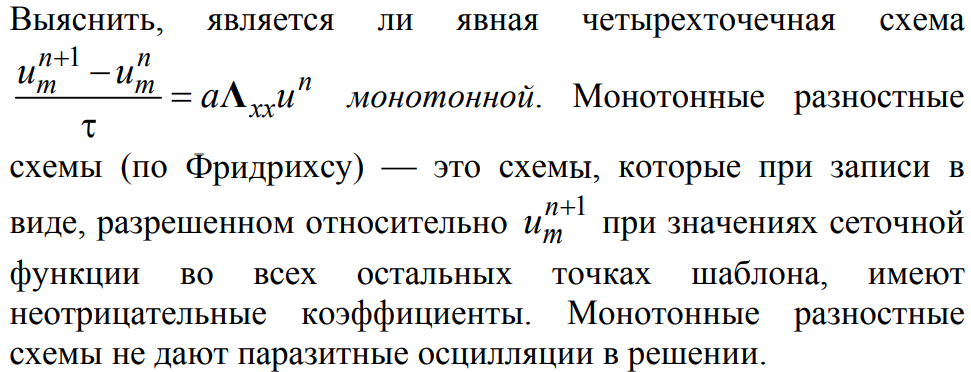
\includegraphics[width=\textwidth]{FRH}
		\end{center}
	\end{figure}
    \vspace{0.5cm}
    \subsubsection{К терминам диссипативная и дисперсионная ошибка}
    
    \begin{figure}[h]
		\begin{center}
			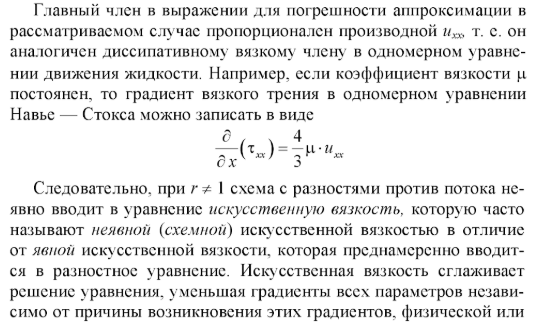
\includegraphics[width=\textwidth, height=16\normalbaselineskip]{diss}
			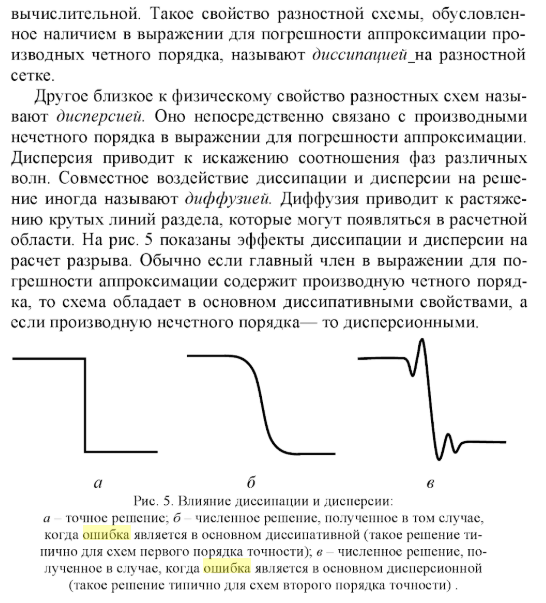
\includegraphics[width=\textwidth, height=22\normalbaselineskip]{disp}
		\end{center}
	\end{figure}
    \newpage
    \newpage
    \subsection{Реализация схемы КИР}
    Какой то неприятный косяк с размером изображений/\\
    Поэтому реализация второй схемы не будет здесь приводится.\\
    Порядок аппроксимации оценен как второй.

    \begin{figure}[h]
		\begin{center}
			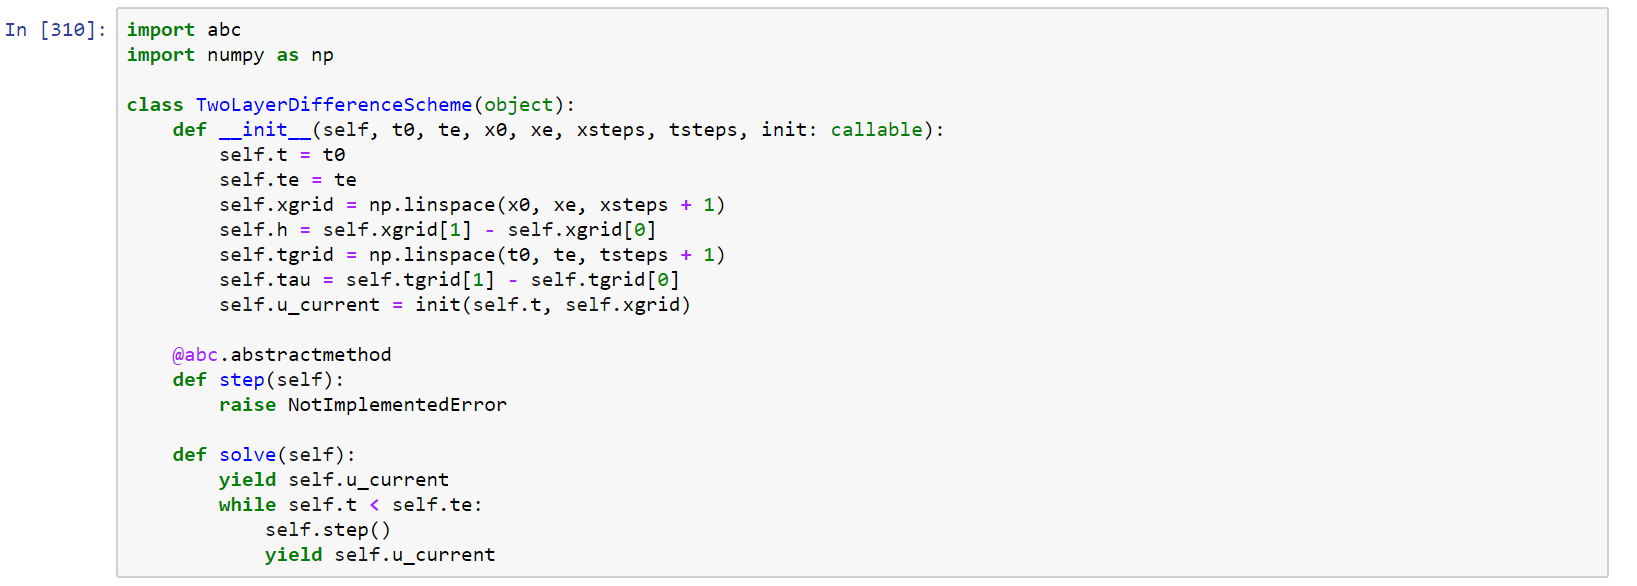
\includegraphics[scale=0.4]{1}
 			\caption{Модель разностной схемы}        
		\end{center}
	\end{figure}
\begin{figure}[h]
		\begin{center}
			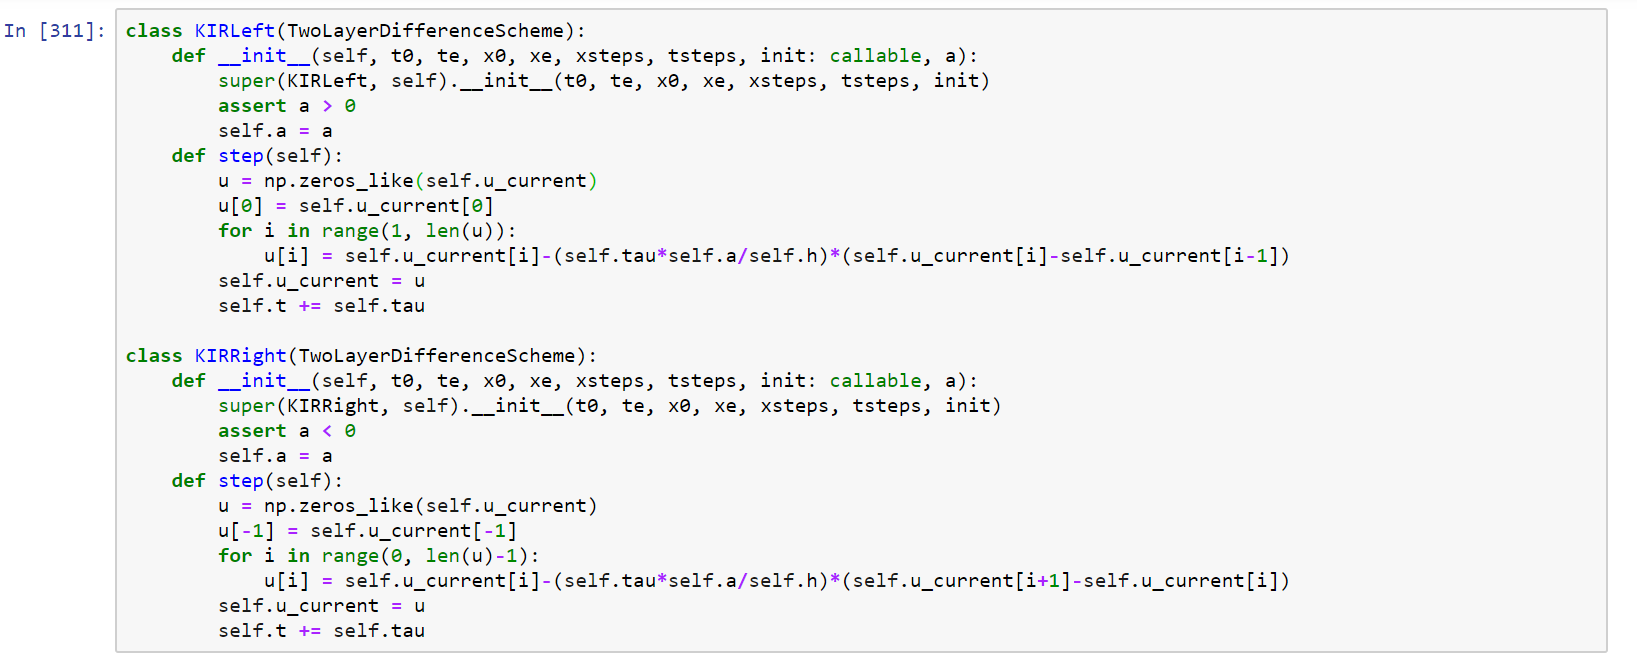
\includegraphics[scale=0.4]{2}
 			\caption{Реализация реккурентного задания u\_n}        
		\end{center}
	\end{figure}

    \newpage
    \subsection{Графики решения}
\begin{figure}[h]
		\begin{center}
			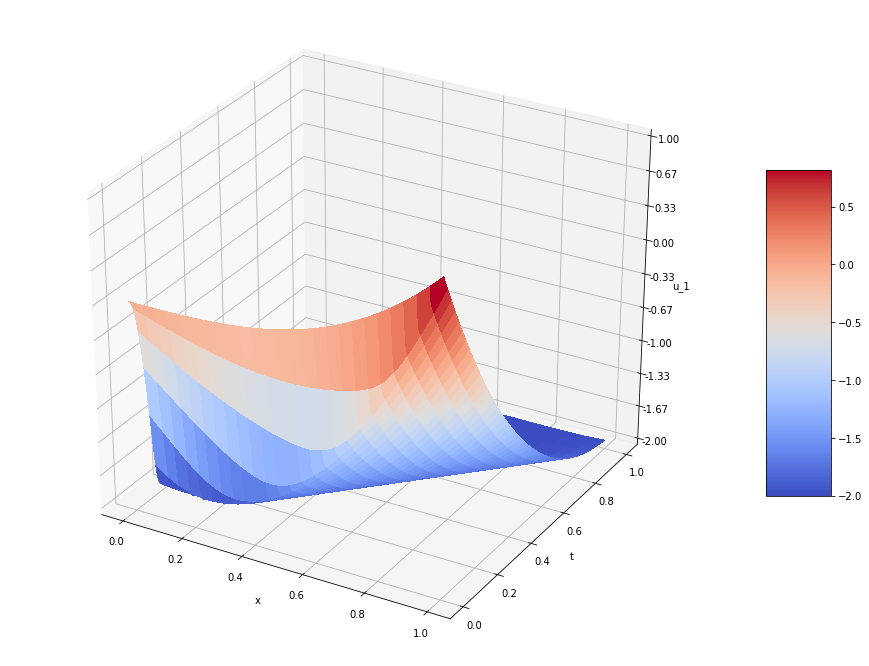
\includegraphics[scale=0.35]{graph1}
			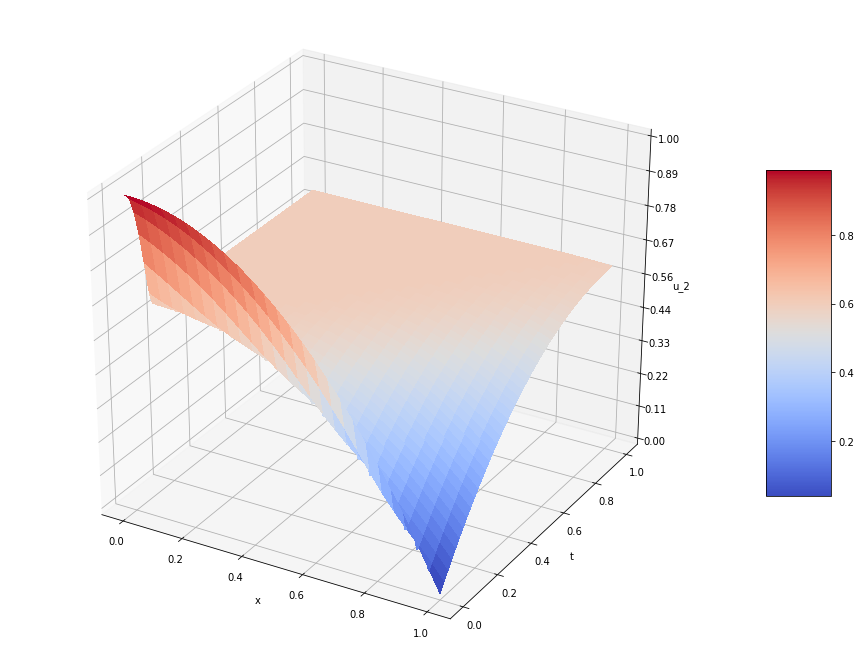
\includegraphics[scale=0.35]{graph2}      
			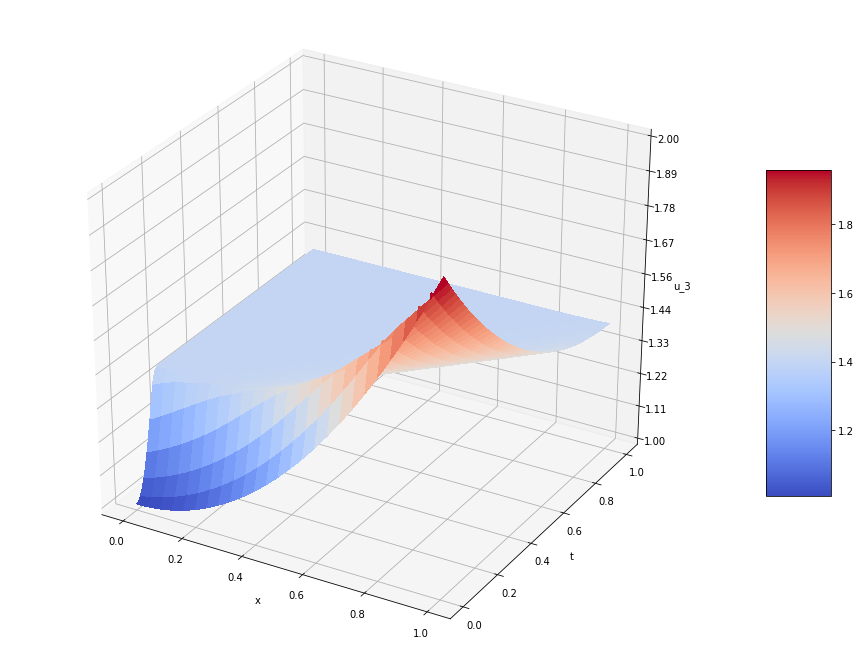
\includegraphics[scale=0.35]{graph3}
			\caption{Схема КИР}           
		\end{center}
	\end{figure}
    
    \subsection{Схема Федоренко}
    \begin{equation}
\frac{u_{m}^{n+1}-u_{m}^{n}}{\tau}+\frac{u_{m}^{n}-u_{m-1}^{n}}{h}+\frac{\gamma}{2 \tau}\left(\frac{a \tau}{h}-\frac{a^{2} \tau^{2}}{h^{2}}\right)\left(u_{m+1}^{n}-2 u_{m}^{n}+u_{m-1}^{n}\right)=0
\end{equation}

\begin{equation}
\gamma=\left\{\begin{array}{ll}{1,} & {\left|y_{m-1}^{n}-2 y_{m}^{n}+y_{m+1}^{n}\right|<\xi\left|y_{m}^{n}-y_{m-1}^{n}\right|} \\ {0,} & {\left|y_{m-1}^{n}-2 y_{m}^{n}+y_{m+1}^{n}\right|>\xi\left|y_{m}^{n}-y_{m-1}^{n}\right|}\end{array}\right.
\end{equation}

Данная схема при обращении анализатора гладкости решения в ноль переходит в схему Куранта-Изаксона-Риса. Всё, что сказано о ней в предыдущей части остаётся справедливым. В случае $\gamma = 1$ получаем схему второго порядка аппроксимации. В первом дифференциальном приближении (в данном отчёте не приводится ввиду громоздкости выкладок) находятся члены с третьей производной, что говорит о преобладании дисперсионной ошибки. Согласно определению Фридрихса, схема не является монотонной.

В отличие от предыдущего случая, для использования данного метода придётся задать граничные условия для обоих концов рассчётного отрезка. Поэтому решения, полученные при помощи предыдущих схем и схемы Федоренко, будут качественно отличаться друг от друга. \\

В рассматриваемом примере при изменении параметра $\xi$ не происходит существенных изменений внешнего вида решений.\\
Далее приводятся графики построенных решений.

\begin{figure}[h]
		\begin{center}
			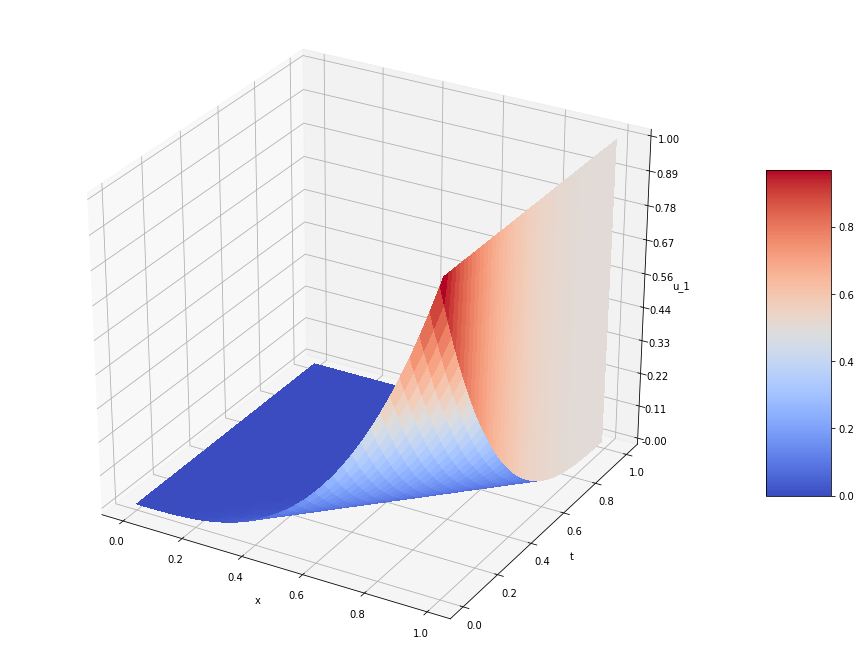
\includegraphics[scale=0.35]{graph4}
			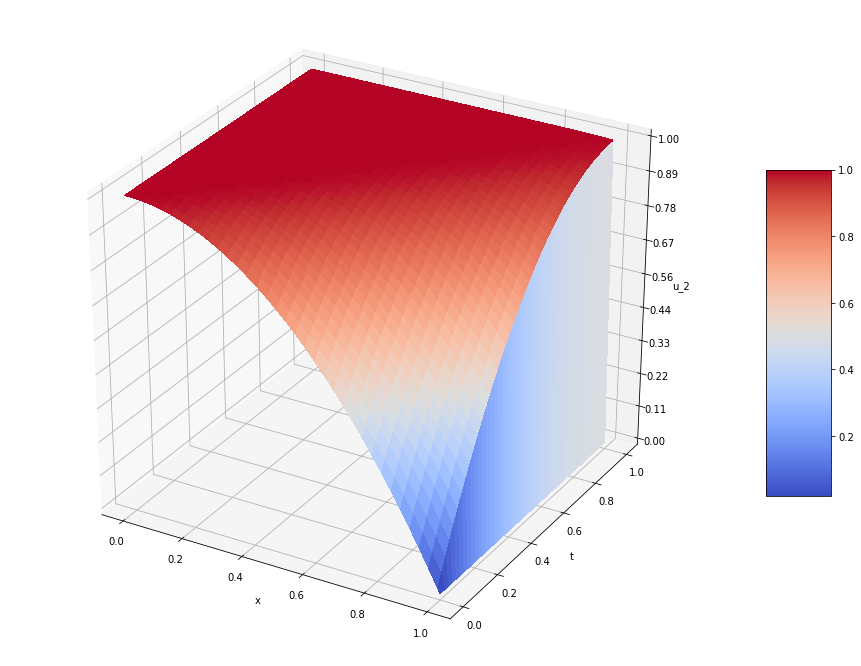
\includegraphics[scale=0.35]{graph5}      
			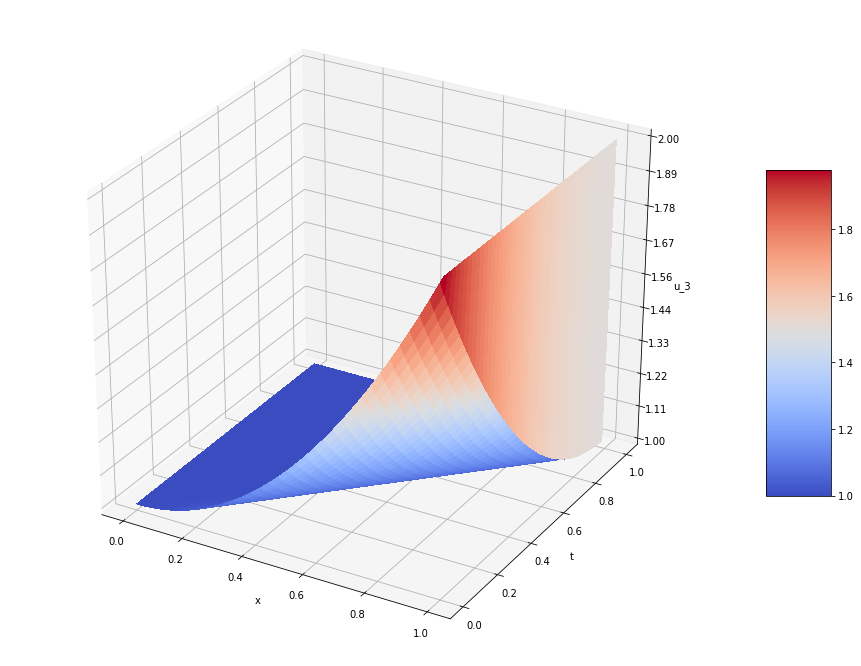
\includegraphics[scale=0.35]{graph6}
			\caption{Гибридная схема Федоренко}           
		\end{center}
	\end{figure}


\end{document}